\section{Experiments}\label{sec:experiments}

\subsection{Experiment details}

To evaluate the RL performance, the merge network(see Fig. \ref{fig:envs}(c)) is chosen as a benchmark. This network is given by the benchmark paper\cite{Vinitsky2018}. In the merge network, there is a highway and an intersection. The intersection can be considered as disturbance to the highway. Due to the disturbance, when the inflow rate reaches to a certain level, stop-and-go wave occurs at the intersection, and it propagates from right to left. The goal of this task is to reduce the stop-and-go wave by controlling 10\% of cars on the road using RL. 

The details of the environment is as follows. To apply multi-agents RL, the states, actions, reward are changed from the benchmark.

\begin{itemize}
    \item States: In this environment, the RL cars can communicate to the leading RL car if it exists, i.e. the state $s$ consists of two parts, the information of the own car$i$ and the information of the leading RL car$i_{\text {lead}}$. The information, $i$ or $i_{lead}$, consists of 6 elements: speeds, bumper-to-bumper distance of the leading and following cars, and the distance to the intersection, i.e. $i := \left(v_{i, \text { lead }}, v_{i, \text { lag }}, h_{i, \text { lead }}, h_{i, \text { lag }}, v_{i}, d\right)$. The state $s$ consists of two information, i.e. $s := (i, i_{\text { lead }})$.
    \item Actions: Action $a$ is the acceleration to the RL car. The action value is bounded by the minimum and maximum acceleration. Then, the action $a$ is $a \in \mathbb{R}_{[a_{\text {min}}, a_{\text {max}}]}$
    \item Reward: The reward function is based on the original benchmark, but slightly changed to support multi-agent. 
    \begin{equation} \label{eq:originR}
r=\left\|v_{\mathrm{des}}\right\|-\| v_{\mathrm{des}}-v(t) \| -\alpha  \max \left[h_{\max }-h_{i}(t), 0\right]
\end{equation}
    Eq. \ref{eq:originR} is the original reward function given by the previous work\cite{Kreidieh2018}. To support multi-agent, a penalty term is added to the reward function, i.e. the reward function is as follows.
\begin{equation} \label{eq:newR}
r=\left\|v_{\mathrm{des}}\right\|-\| v_{\mathrm{des}}-v(t) \| -\alpha \max \left[h_{\max }-h_{i}(t), 0\right] - c
\end{equation}
    Compared to the original reward function, $c \in \mathcal{R}$ is subtracted from the reward function. This penalty term makes the agent get out from the highway as fast as it can.

    In this research, the values of the parameters are $v_{\mathrm{des}} = 25$, $h_{\max } = 10$, $c = 1.0$

    \item Traffic information:
    \begin{itemize}
        \item Inflow rate of the highway: 2000 veh/hr
        \item Inflow rate of the disturbance: 100 veh/hr
        \item RL car ratio: 10\%
    \end{itemize}
\end{itemize}

The detail of the training is as follows. The agent of the GAIL is updated by PPO.

\begin{itemize}
    \item PPO model: 

    \begin{itemize}
        \item hidden layers: (128, 64, 32)
        \item GAE\cite{Schulman2015} lambda: 0.97
        \item learning rate: $5\times 10^{-4}$
    \end{itemize}

    \item GAIL discriminator:
    
    \begin{itemize}
        \item hidden layers: (128, 128)
        \item learning rate: 0.005
    \end{itemize}

    \item training:

    \begin{itemize}
        \item number of cpus: 20
        \item training iteration(PPO): 50
        \item training iteration(GAIL): 150
    \end{itemize}
\end{itemize}

\subsection{Results}

Fig. \ref{fig:congestion} shows how much congestion occurs on the highway. In the situation without any RL cars, the congestion occurred at the intersection and it propagates as a stop-and-go wave. On the other hand, the PPO and GAIL agents successfully reduce the congestion. 

Fig. \ref{fig:outflow} and \ref{fig:velocity} show the velocity and the outflow rate of the highway. Without RL, the mean velocity decreases and converges about 8 m/s around 300 steps. On the other hand, the trained PPO and GAIL keep the speed around 15 m/s. The PPO agent increases the velocity of the traffic about 40\% with almost the same outflow rate(see Table. \ref{tb:mean}).

The GAIL agent uses the trained PPO agent as the expert. Even though the GAIL agent is not trained on the reward function\ref{eq:newR}, the performance and the behavior of the GAIL agent is pretty similar to that of the PPO agent. The GAIL agent success fully reduce the congestion(Fig. \ref{fig:congestion}) and increase the velocity(Fig. \ref{fig:velocity}).

Since the inflow rate is set as 2000 veh/hr, the outflow rate should be 2000 veh/hr. However, the measured outflow rate is almost 75\% of the inflow rate. This phenomenon is due to the system of the simulator. The simulator stops inserting new cars if cars exist at the start point of the highway. The agent learns how to reduce the inflow rate by waiting at the start point. This reducing traffic effect is similar to the ramp metering on the highway. 


\begin{table}[H] 
\centering
\begin{tabular}{|c|c|c|c|}
\hline
                                                                & No RL & PPO  & GAIL \\ \hline
\begin{tabular}[c]{@{}c@{}}Mean Velocity\\ (m/s)\end{tabular}   & 10.1  & 14.0 & 13.5 \\ \hline
\begin{tabular}[c]{@{}c@{}}Outflow rate\\ (veh/hr)\end{tabular} & 1421  & 1497 & 1551 \\ \hline
\end{tabular}
\caption{Mean velocity and outflow rate by one episode. PPO and GAIL achieve high velocity while keeping almost the same outflow rate.}
\label{tb:mean}
\end{table}

\begin{figure}[]
    \begin{center}
    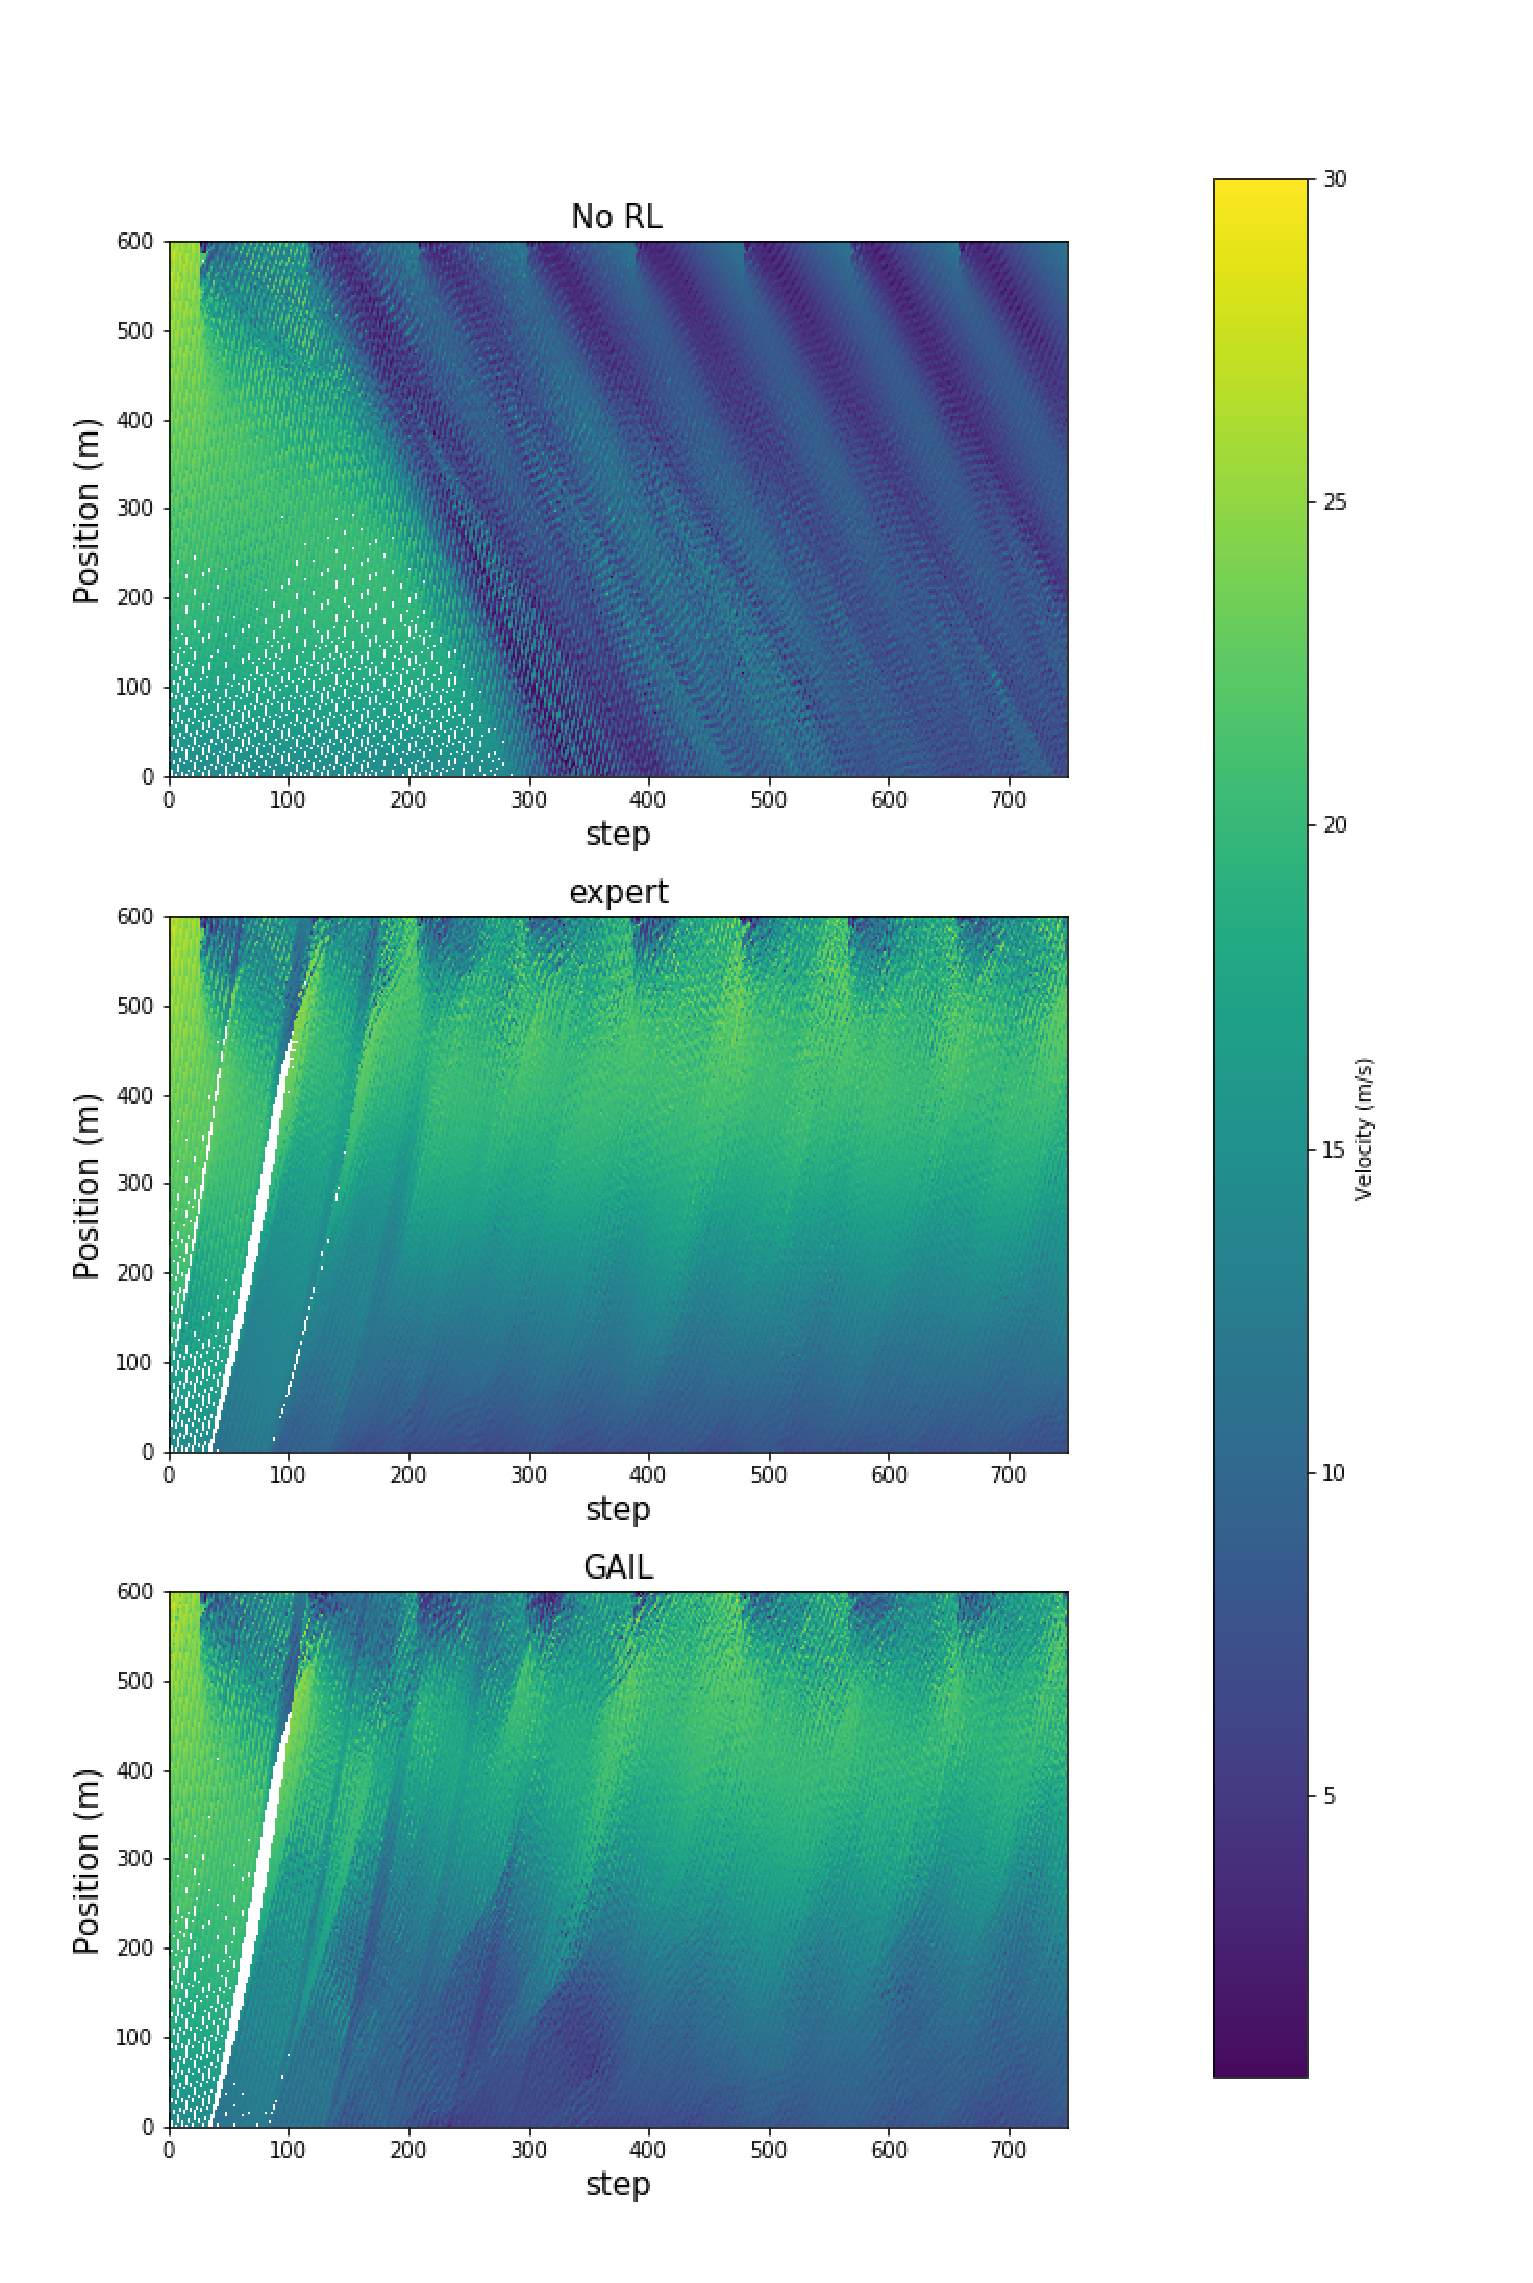
\includegraphics[width=10cm]{img/congestion.eps}
    \caption{Heat map of congestion level on the road. The results are averaged by 50 episodes. From top, the figures are the results of "No RL", "PPO" and "GAIL". If there are slow cars on the road, it appears as blue part. The "No RL" result has stop-and-go waves as blue lines propagating from top left to bottom right, but the other results doesn't have that.}
    \label{fig:congestion}
    \end{center}
\end{figure}

\begin{figure}[]
    \begin{center}
    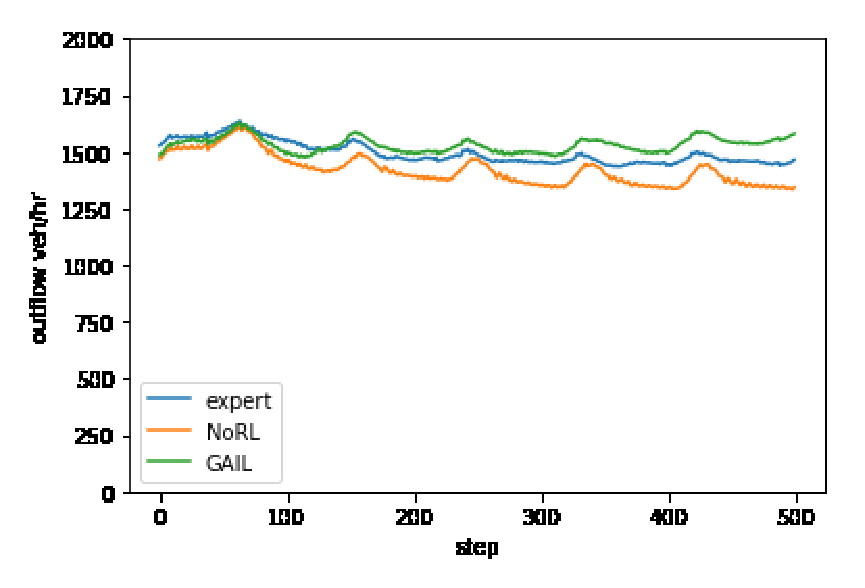
\includegraphics[width=9cm]{img/outflow.eps}
    \caption{Outflow rate during one episode. The results are averaged by 50 episodes. These three results keep almost the same outflow rate, around 1500 veh/hr.}
    \label{fig:outflow}
    \end{center}
\end{figure}

\begin{figure}[]
    \begin{center}
    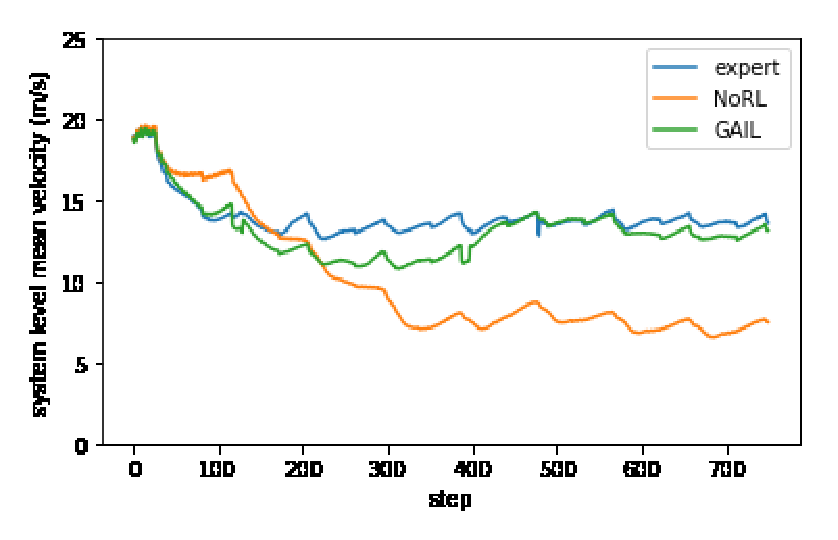
\includegraphics[width=9cm]{img/velocity.eps}
    \caption{Mean velocity of the traffic. The results are averaged by 50 episodes. Compared to the result of "No RL", GAIL and PPO keep high velocity during the episode.}
    \label{fig:velocity}
    \end{center}
\end{figure}
